% Generated by ICLR_Q4.py from experiment_logs_Q4 -- Dubins4D_x0set: Abstract states ($|S|$)
% Shaded band = min/max over seeds; line = median over seeds.
% Picture width is exactly \linewidth. Requires \usepackage{pgfplots}.
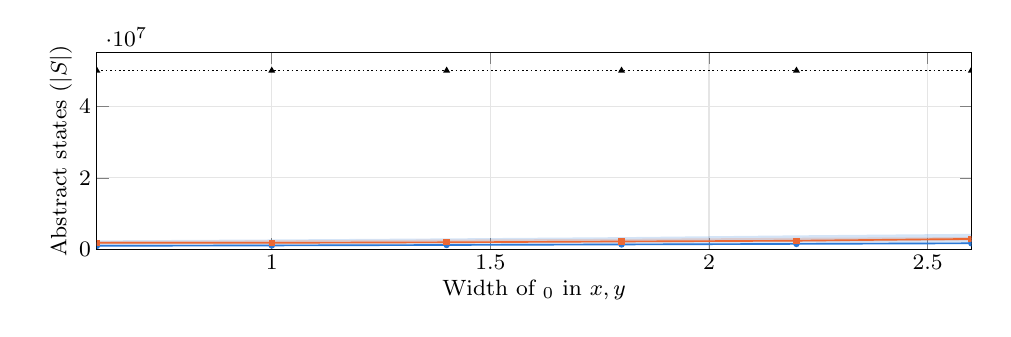
\begin{tikzpicture}[baseline=(current axis.south)]
\definecolor{q4ppo}{RGB}{42,120,214}
\definecolor{q4sac}{RGB}{235,104,52}
\definecolor{q4dense}{RGB}{0,0,0}
\begin{axis}[
    scale only axis, width=\linewidth-25pt-4pt, height=2.5cm,
    xlabel={Width of $\X_0$ in $x,y$},
    ylabel={Abstract states ($|S|$)}, ylabel style={align=center},
    xmin=0.6, xmax=2.6, xtick={1,1.5,2,2.5},
    ymin=0,
    grid=major, grid style={gray!20}, clip marker paths=true,
    label style={font=\footnotesize}, tick label style={font=\footnotesize, inner sep=2pt},
    xlabel shift=-2pt, ylabel shift=-3pt,  % labels close to the tick labels
]
% PPO: 5 seeds per X0 span
\addplot[draw=none, fill=q4ppo, fill opacity=0.2, forget plot] coordinates {(0.6,904151) (1,1.01892e+06) (1.4,1.15981e+06) (1.8,1.32139e+06) (2.2,1.50771e+06) (2.6,1.68467e+06) (2.6,4.37335e+06) (2.2,3.95113e+06) (1.8,3.45003e+06) (1.4,3.1016e+06) (1,2.79997e+06) (0.6,2.54632e+06)} -- cycle;
\addplot[q4ppo, semithick, mark=*, mark size=0.85pt] coordinates {(0.6,1.0237e+06) (1,1.13097e+06) (1.4,1.25874e+06) (1.8,1.40682e+06) (2.2,1.56507e+06) (2.6,1.73367e+06)};
% SAC: 2/5 seeds per X0 span
\addplot[draw=none, fill=q4sac, fill opacity=0.2, forget plot] coordinates {(0.6,1.56618e+06) (1,1.70914e+06) (1.4,1.81878e+06) (1.8,1.97282e+06) (2.2,2.15849e+06) (2.6,2.46615e+06) (2.6,3.46406e+06) (2.2,3.2765e+06) (1.8,2.96682e+06) (1.4,2.75992e+06) (1,2.55642e+06) (0.6,2.28302e+06)} -- cycle;
\addplot[q4sac, semithick, mark=square*, mark size=0.85pt] coordinates {(0.6,1.88455e+06) (1,1.86944e+06) (1.4,2.01058e+06) (1.8,2.24076e+06) (2.2,2.44937e+06) (2.6,2.9651e+06)};
% Dense (single deterministic run per X0 span)
% No dense run for X0 span(s) 0.6, 1, 1.4, 1.8, 2.2, 2.6: there, the number of cells of the dense grid (100x50x100x100) is plotted
\addplot[q4dense, semithick, mark=triangle*, mark size=0.85pt, densely dotted, mark options={solid}] coordinates {(0.6,5e+07) (1,5e+07) (1.4,5e+07) (1.8,5e+07) (2.2,5e+07) (2.6,5e+07)};
\end{axis}
% Fix the bounding box to exactly \linewidth wide: the axis box plus the label margins
\path (current axis.south west |- current bounding box.south) ++(-25pt,0) coordinate (q4sw)
      (current axis.north east |- current bounding box.north) ++(4pt,0) coordinate (q4ne);
\pgfresetboundingbox
\useasboundingbox (q4sw) rectangle (q4ne);
\end{tikzpicture}%
